% theory.tex -- dronelocate: mathematics, algorithms, architecture
% Build:  pdflatex theory.tex  (twice, for cross-references)
\documentclass[11pt,a4paper]{article}

\usepackage[T1]{fontenc}
\usepackage[utf8]{inputenc}
\usepackage{lmodern}
\usepackage{microtype}
\usepackage[margin=2.4cm]{geometry}
\usepackage{amsmath,amssymb}
\usepackage{booktabs}
\usepackage{array}
\usepackage{xcolor}
\usepackage{tikz}
\usepackage{caption}
\usepackage{enumitem}
\usepackage[hidelinks]{hyperref}

\usetikzlibrary{positioning,arrows.meta,shapes.geometric,fit,backgrounds,calc}

\definecolor{accent}{RGB}{0,90,140}
\definecolor{warn}{RGB}{150,40,20}
\definecolor{soft}{RGB}{240,244,248}
\definecolor{softrule}{RGB}{180,196,210}

\newcommand{\code}[1]{\texttt{\small #1}}
\newcommand{\uvec}[1]{\hat{\mathbf{#1}}}
\newcommand{\R}{\mathbb{R}}
\DeclareMathOperator{\median}{median}
\DeclareMathOperator*{\argmax}{arg\,max}
\DeclareMathOperator*{\argmin}{arg\,min}
\DeclareMathOperator{\diag}{diag}
\DeclareMathOperator{\sinc}{sinc}

% boxed remark
\newenvironment{keypoint}
  {\par\medskip\noindent\begin{tikzpicture}\node[draw=softrule,fill=soft,
    rounded corners=2pt,inner sep=8pt,text width=\dimexpr\linewidth-20pt\relax,
    align=justify]\bgroup\begin{minipage}{\dimexpr\linewidth-20pt\relax}\small}
  {\end{minipage}\egroup;\end{tikzpicture}\par\medskip}

\title{\textbf{Passive RF Localization of Non-Cooperative Drones}\\[2mm]
       \large Mathematics, Algorithms and System Architecture}
\author{\normalsize dronelocate --- technical reference}
\date{\normalsize\today}

\begin{document}
\maketitle

\begin{abstract}
\noindent
This document describes the theory and implementation of a passive
time-difference-of-arrival (TDOA) localization system for non-cooperative
drones. Ten sensor nodes observe the drone's own radio emissions, stream
compressed IQ to a central supernode over a publish/subscribe bus, and the
supernode cross-correlates the captures, solves a three-dimensional position
by weighted nonlinear least squares, and tracks it with a Kalman filter. The
treatment covers coordinate frames and dilution of precision, the signal and
clock models, detection (energy and cyclostationary), time-delay estimation
(band-limited interpolation, the cross-ambiguity function, and generalised
cross-correlation weighting), the position solver (grid-seeded Gauss--Newton
with robust loss, an altitude prior, and generalised least squares over all
node pairs), and the tracking filter including tightly coupled updates from
under-determined bursts. A final section collects the numerical-conditioning
failures encountered during development, several of which cost more accuracy
than any algorithmic choice discussed here.
\end{abstract}

\tableofcontents

%==================================================================
\section{Problem statement}

A drone that transmits --- video downlink, control uplink, telemetry --- can
be located from its own emissions, with no cooperation and no transmission
from the sensor network. This is the passive, or \emph{silent}, case: the
sensors radiate nothing and are therefore neither detectable nor jammable by
the target.

Let the emitter be at unknown position $\mathbf{x}\in\R^3$ and let sensor
node $i$ occupy known position $\mathbf{n}_i\in\R^3$. A signal leaving the
emitter at unknown time $t_0$ arrives at node $i$ at

\begin{equation}
  t_i \;=\; t_0 \;+\; \frac{\lVert \mathbf{x}-\mathbf{n}_i\rVert}{c}
        \;+\; \varepsilon_i ,
  \label{eq:arrival}
\end{equation}

where $c$ is the speed of light and $\varepsilon_i$ is node $i$'s clock
error relative to a common timebase. The emission time $t_0$ is unknown and
uninteresting, so it is eliminated by differencing pairs of arrivals:

\begin{equation}
  \tau_{ij} \;=\; t_i - t_j
  \;=\; \frac{\lVert \mathbf{x}-\mathbf{n}_i\rVert
             -\lVert \mathbf{x}-\mathbf{n}_j\rVert}{c}
        \;+\; (\varepsilon_i-\varepsilon_j).
  \label{eq:tdoa}
\end{equation}

Each measured $\tau_{ij}$ constrains $\mathbf{x}$ to one sheet of a
hyperboloid of revolution with foci $\mathbf{n}_i,\mathbf{n}_j$. Three
independent constraints fix a point in space; more than three
over-determine it and permit a least-squares solution with a covariance.

Two facts drive the entire design. First, $c\approx
0.3\,\text{m}/\text{ns}$, so a timing error of one nanosecond is thirty
centimetres of range error --- and the residual clock term
$\varepsilon_i-\varepsilon_j$ in~\eqref{eq:tdoa} enters with exactly the
same weight as geometry. Timing discipline, not signal processing, sets the
achievable accuracy. Second, $\tau_{ij}$ must be \emph{measured}, which
requires the same emission to be recognisable in two different receivers'
samples; that measurement is a cross-correlation, and everything in
Section~\ref{sec:tde} exists to make it unbiased.

%==================================================================
\section{System architecture}

\subsection{Topology and data flow}

Figure~\ref{fig:arch} shows the deployment. Nodes are thin: they capture,
detect, buffer, and announce. The supernode holds all the geometry and makes
all the decisions.

\begin{figure}[htbp]
\centering
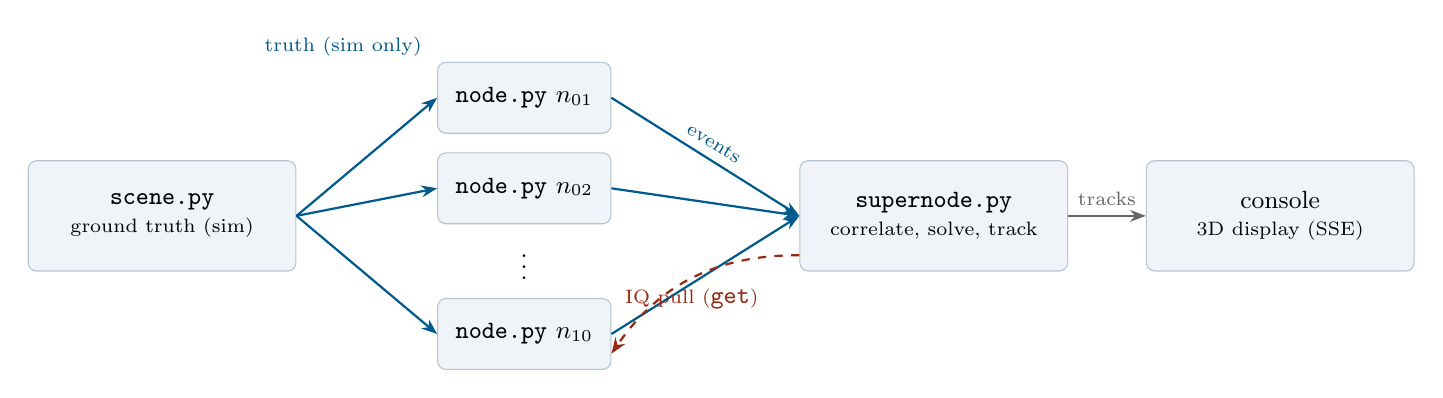
\begin{tikzpicture}[
  font=\small,
  box/.style={draw=softrule,fill=soft,rounded corners=3pt,minimum height=9mm,
              inner xsep=6pt,align=center},
  node1/.style={box,minimum width=22mm},
  big/.style={box,minimum width=34mm,minimum height=14mm},
  ev/.style={-{Stealth[length=2mm]},accent,thick},
  iq/.style={-{Stealth[length=2mm]},warn,thick,dashed},
  tr/.style={-{Stealth[length=2mm]},black!60,thick},
]
\node[big] (scene) at (0,0) {\code{scene.py}\\[-1pt]\scriptsize ground truth (sim)};
\node[node1] (n1) at (4.6,1.5) {\code{node.py} $n_{01}$};
\node[node1] (n2) at (4.6,0.35) {\code{node.py} $n_{02}$};
\node[minimum width=22mm] (dots) at (4.6,-0.55) {$\vdots$};
\node[node1] (n3) at (4.6,-1.5) {\code{node.py} $n_{10}$};
\node[big] (sup) at (9.8,0) {\code{supernode.py}\\[-1pt]\scriptsize correlate, solve, track};
\node[big] (con) at (14.2,0) {console\\[-1pt]\scriptsize 3D display (SSE)};

\draw[ev] (scene.east) -- (n1.west);
\draw[ev] (scene.east) -- (n2.west);
\draw[ev] (scene.east) -- (n3.west);
\draw[ev] (n1.east) -- node[above,sloped,font=\scriptsize]{events} (sup.west);
\draw[ev] (n2.east) -- (sup.west);
\draw[ev] (n3.east) -- (sup.west);
\draw[iq] ($(sup.west)+(0,-0.5)$) to[bend right=28]
      node[below,font=\scriptsize,pos=0.5]{IQ pull (\code{get})} ($(n3.east)+(0,-0.25)$);
\draw[tr] (sup.east) -- node[above,font=\scriptsize]{tracks} (con.west);

\node[font=\scriptsize,text=accent,align=center] at (2.3,2.15) {truth (sim only)};
\end{tikzpicture}
\caption{Star topology. The supernode listens; nodes connect as clients.
Solid arrows are small, frequent, never-dropped messages; the dashed arrow
is the bulk IQ transfer, which is \emph{pulled} on demand.}
\label{fig:arch}
\end{figure}

\subsection{Pull, do not push}
\label{sec:pull}

A node hears a burst, computes a detection event of roughly one kilobyte,
and publishes that. The IQ itself --- $47$\,kB per $10$\,ms snippet at
$2.4$\,Msps in \code{ci8} --- stays in the node's ring buffer. The supernode
groups the events belonging to one burst, chooses a geometrically favourable
subset of the nodes that heard it, and issues a query only to those.

Ten nodes typically hear a burst and six or seven are queried. Halving the
transfers costs nothing in accuracy because the discarded nodes were
geometrically redundant --- the selection criterion in
Section~\ref{sec:gdop} makes that statement precise.

\subsection{Quality of service}

The bus carries traffic with incompatible requirements, so each key
expression is assigned a priority and a congestion policy:

\begin{center}
\begin{tabular}{@{}llll@{}}
\toprule
\textbf{Key expression} & \textbf{Priority} & \textbf{Congestion} & \textbf{Purpose}\\
\midrule
\code{dc/\{site\}/\{node\}/evt/detect} & interactive high & block & $\sim$1\,kB events\\
\code{dc/\{site\}/\{node\}/iq}         & background       & block & IQ queryable (pull)\\
\code{dc/\{site\}/\{node\}/health}     & data low         & drop  & telemetry\\
\code{dc/\{site\}/cmd/\{node\}}        & interactive high & block & retasking\\
\code{dc/\{site\}/track/live}          & data high        & block & fused tracks\\
\code{dc/\{site\}/sim/truth}           & ---              & ---   & \textbf{simulation only}\\
\bottomrule
\end{tabular}
\end{center}

The priority split is what stops a $47$\,kB bulk transfer from delaying a
one-kilobyte detection event. Health telemetry \emph{drops} rather than
blocking, because a stale health message is worthless and must never apply
backpressure to the pipeline.

\begin{keypoint}
\textbf{Design invariant.} Nothing on the solve path reads the ground-truth
channel. Emulated nodes subscribe to it to render \emph{their own} IQ ---
each applying its own geometric delay, clock error, path loss and noise ---
then discard it and publish only detections. The supernode does subscribe,
but exclusively to score the answer in metres for the display. Delete that
key expression and the system still localizes, merely unscored. This is what
makes the simulation an honest test rather than a demonstration.
\end{keypoint}

The same separation governs the display. The console can drape
OpenStreetMap raster tiles and extruded building footprints over the survey
plane, and can re-centre that basemap on any of several cities. All of it is
decoration: no measurement is taken against it, the buildings are drawn at a
default height wherever the source has no surveyed one, and the map's
coordinate conversion is a flat tangent-plane approximation rather than the
ellipsoidal transform of Section~\ref{sec:frames}. Re-centring the basemap
moves the streets under the constellation, not the constellation --- sensor
positions are metres in a local frame and do not depend on which city is
drawn beneath them.

%==================================================================
\section{Coordinate frames and geometry}
\label{sec:frames}

\subsection{WGS84 to local tangent plane}

All estimation runs in a local East--North--Up (ENU) Cartesian frame in
metres. Geodetic coordinates appear only at the configuration boundary and
at the display boundary. Least squares performed in degrees introduces a
direction-dependent bias, because a degree of longitude and a degree of
latitude are different distances, and that anisotropy would be absorbed
silently into the position estimate.

Geodetic to Earth-Centred Earth-Fixed, with semi-major axis $a$, flattening
$f$, and $e^2=f(2-f)$:
\begin{align}
  N(\varphi) &= \frac{a}{\sqrt{1-e^{2}\sin^{2}\varphi}}, \\
  \mathbf{p}_{\text{ECEF}} &=
  \begin{bmatrix}
    (N+h)\cos\varphi\cos\lambda\\
    (N+h)\cos\varphi\sin\lambda\\
    \bigl(N(1-e^{2})+h\bigr)\sin\varphi
  \end{bmatrix}.
\end{align}

With a site origin $(\varphi_0,\lambda_0,h_0)$ the rotation into ENU is
\begin{equation}
  \mathbf{R} =
  \begin{bmatrix}
    -\sin\lambda_0 & \cos\lambda_0 & 0\\
    -\sin\varphi_0\cos\lambda_0 & -\sin\varphi_0\sin\lambda_0 & \cos\varphi_0\\
     \cos\varphi_0\cos\lambda_0 &  \cos\varphi_0\sin\lambda_0 & \sin\varphi_0
  \end{bmatrix},
  \qquad
  \mathbf{p}_{\text{ENU}} = \mathbf{R}\,(\mathbf{p}_{\text{ECEF}}-\mathbf{p}_{0,\text{ECEF}}).
\end{equation}
The inverse uses Bowring's iteration, which converges to sub-millimetre at
these altitudes in a handful of steps.

\subsection{Dilution of precision}
\label{sec:gdop}

Linearising~\eqref{eq:tdoa} about a candidate position gives the measurement
Jacobian. With $\uvec{u}_i$ the unit vector from the target toward node $i$,
the row for the pair $(i,\text{ref})$ is $\uvec{u}_{\text{ref}}-\uvec{u}_i$.
Collecting the rows into $\mathbf{H}$, the geometric covariance factor is
$(\mathbf{H}^\top\mathbf{H})^{-1}$, whence
\begin{equation}
  \text{HDOP}=\sqrt{C_{11}+C_{22}},\qquad
  \text{VDOP}=\sqrt{C_{33}},\qquad
  \text{PDOP}=\sqrt{\operatorname{tr}\mathbf{C}},
  \qquad \mathbf{C}=(\mathbf{H}^\top\mathbf{H})^{-1}.
\end{equation}

Position error is approximately $\text{DOP}\times c\,\sigma_t$. For the
reference ten-node layout, $\text{HDOP}\approx0.59$ while
$\text{VDOP}\approx16.4$. That ratio is not a defect of the solver: with
eight of ten nodes near ground level, every measurement row is nearly
horizontal and the vertical component of $\mathbf{x}$ is weakly observable.
Two nodes are deliberately elevated ($45$\,m and $70$\,m) to break the
coplanarity; setting them back to ground level roughly triples the vertical
error. \emph{Vertical accuracy is bought with mast height, not with
software.}

\subsection{Node selection}

Given the set $\mathcal{H}$ of nodes that heard a burst, the supernode
chooses a subset $\mathcal{S}\subseteq\mathcal{H}$ of bounded size that
minimises PDOP. The search is greedy: seed with the strongest node by SNR,
then repeatedly add whichever candidate most reduces PDOP evaluated at a
provisional target position. That position is an RSSI-weighted centroid,
\begin{equation}
  \mathbf{x}_{\text{seed}}
  = \frac{\sum_{i\in\mathcal{H}} w_i \mathbf{n}_i}{\sum_{i\in\mathcal{H}} w_i},
  \qquad w_i = 10^{\,\text{RSSI}_i/20},
\end{equation}
with the vertical component replaced by the configured altitude prior. The
seed only has to be good enough to \emph{rank} geometries, and RSSI is
already present in the event, so it costs nothing.

\paragraph{How much geometry is enough.} Selection only pays if adding
sensors actually buys dilution, and for this constellation it stops paying
early. Evaluated at the orbit centre, over every subset containing an
elevated node:

\begin{center}
\begin{tabular}{@{}lrrr@{}}
\toprule
\textbf{Sensors} & \textbf{HDOP} & \textbf{VDOP} & \textbf{PDOP}\\
\midrule
all 10      & 0.62 & 10.83 & 10.85\\
best 7      & 0.83 & 11.05 & 11.08\\
best 6      & 0.99 & 11.11 & 11.16\\
best 5      & 3.21 & 12.41 & 12.82\\
\bottomrule
\end{tabular}
\end{center}

Seven of ten is indistinguishable from ten, six is close behind, and five
falls off a cliff --- HDOP nearly quadruples, because at five the survivors
no longer surround the target and the horizontal problem becomes
one-sided. The vertical barely moves throughout, which is the same point as
Section~\ref{sec:gdop} from the other direction: VDOP here is set by the
sensors' \emph{elevation spread}, not by how many of them there are, so
adding ground-level sensors cannot fix it.

Two practical consequences. First, the cap on $|\mathcal{S}|$ is not a
compromise: pulling IQ from more than about seven well-chosen nodes buys
nothing measurable, which is what makes the pull-not-push architecture of
Section~\ref{sec:pull} free rather than lossy. Second, and less obviously,
\emph{configuring} more emulated nodes than the cap is pure waste --- the
surplus render a full signal chain, run detection and publish events that
are never queried. On a constrained machine that is around a third of the
simulation's cost for no geometric return.

%==================================================================
\section{Signal and channel model}

The simulator exists to test the estimator, so it must reproduce every
effect that can bias the estimator --- and be honest about the ones it does
not model.

\subsection{Emitted waveform}

Each node synthesises the emitted burst independently from the burst
identifier, so all nodes agree on the waveform without ever exchanging it.
Two waveform families are available.

\paragraph{Band-limited Gaussian noise.} A filtered complex Gaussian burst
has a near-ideal thumbtack autocorrelation, so correlation quality tracks
SNR rather than waveform structure. This isolates solver behaviour, and is
the right choice when the question is about geometry or timing.

\paragraph{CP-OFDM.} The realistic case. A drone video downlink is OFDM, so
the synthetic emitter builds $N_{\text{sym}}$ symbols with $N_u=128$ useful
samples and a cyclic prefix of $N_{cp}=16$:
\begin{equation}
  s_m[n] = \frac{1}{N_u}\sum_{k\in\mathcal{K}} X_{m,k}\,
           e^{\,j2\pi kn/N_u},\qquad n=-N_{cp},\dots,N_u-1,
\end{equation}
with $X_{m,k}$ QPSK on the active carriers $\mathcal{K}$, pilots at fixed
positions every eighth carrier, and a DC null. At $2.4$\,Msps this is
$18.75$\,kHz carrier spacing, adjacent to the LTE family that commercial
drone links resemble.

The distinction matters more than it appears. \emph{A flat spectrum makes
whole classes of technique inexpressible}: spectral weighting
(Section~\ref{sec:gcc}) degenerates to a constant, and cyclostationary
detection (Section~\ref{sec:cyclo}) has no cyclic structure to find. An
algorithm validated against white noise is validated against nothing.

\begin{keypoint}
\textbf{Pilots must be scrambled, and the reason is a delay-estimation
hazard rather than a communications one.} Repeating an identical pilot
vector on every symbol makes the waveform periodic at the symbol rate,
which places autocorrelation sidelobes at multiples of $N_u+N_{cp}$ at some
$17\%$ of the main peak. Whether that matters depends entirely on the
sample rate: at $2.4$\,Msps one symbol is $60\,\mu$s and the sidelobes fall
outside a $\pm30\,\mu$s search window, while at $20$\,Msps a symbol is
$7.2\,\mu$s and they fall well inside it --- where a correlator will
occasionally lock onto one and return a confident lag wrong by an exact
multiple of the symbol period. The pilots therefore carry a per-symbol BPSK
scrambling sequence, as real OFDM does. Per-subcarrier power is unchanged,
so the spectrum keeps its pilot structure for weighting, and the cyclic
prefix is untouched, so the detector of Section~\ref{sec:cyclo} is
unaffected; measured sidelobes fall roughly twentyfold. Note the general
form of the lesson: \emph{a narrowband test cannot see this defect at all},
because the artefact only enters the search window once the capture is
wide.
\end{keypoint}

\subsection{Frequency hopping}
\label{sec:hop}

A real datalink does not sit still. It hops across the band on a schedule
the receiver is not told, so the emitter transmits at $f_c + \delta_b$ for
burst $b$, and in a node's baseband the burst appears at $\delta_b$ rather
than at DC. Energy shifted beyond the digitized band never reaches the ADC
at all --- the analog front end removes it --- so a hop outside the window
does not arrive attenuated, it does not arrive.

That distinction is what makes hopping more dangerous than any effect
considered so far. Every other impairment in this document degrades a
measurement; this one deletes it, and a missed detection cannot be
recovered downstream by weighting, gating or robust loss. Measured against
a $17.5$\,MHz hop span, a $2.4$\,Msps node detects $1$ burst in $16$, with
a median post-hop SNR of $-106$\,dB. Section~\ref{sec:chan} is the
receiver-side answer.

In the simulator the hop is derived from the burst identifier, so every
node renders the same hop without exchanging anything --- the same
coordination-free construction as the waveform itself --- while the
receiver is told nothing and must find the energy for itself.

\subsection{Multipath}
\label{sec:multipath}

Free-space propagation gives each node exactly one arrival. A real site
adds reflections, so node $i$ observes
\begin{equation}
  y_i[n] = \sum_{\ell=0}^{L} a_{i\ell}\; s\!\left(n - \Delta_i
           - f_s\,\tau_{i\ell}\right) + \nu_i[n],
  \qquad \tau_{i0}=0,
\end{equation}
with excess delays $\tau_{i\ell}>0$ drawn from an exponential power-delay
profile and total echo power a Rician $K$ below the direct path. The
reflectors are buildings and terrain, so the profile is a property of the
node's location: it is drawn once and held, not redrawn per burst. That
choice is the whole point. A per-burst redraw would average away over a
run and appear as noise; a static profile biases every measurement from
that node in the same direction, forever.

The consequences are developed in Section~\ref{sec:mp-effect}, but the
signature is worth stating with the model: multipath produces a large
\emph{bias} while leaving \emph{precision} untouched. The measurement is
exactly as repeatable as it was before, and simply wrong.

\subsection{Propagation and receiver}

Node $i$'s baseband capture over a window beginning at $t_{\text{cap}}$ is
\begin{equation}
  y_i[n] = A_i\, g[n]\, s\!\left(n - \Delta_i\right)
           e^{\,j(2\pi f_{d,i} n/f_s + \phi_i)} + \nu_i[n] + \iota_i[n],
  \label{eq:rx}
\end{equation}
with the fractional sample delay
\begin{equation}
  \Delta_i = f_s\Bigl[(t_0-t_{\text{cap}}) + \frac{r_i}{c} + \varepsilon_i\Bigr],
  \qquad r_i=\lVert\mathbf{x}-\mathbf{n}_i\rVert .
  \label{eq:delay}
\end{equation}
Here $A_i$ is free-space amplitude ($\propto 1/r_i$), $g[n]$ a raised-cosine
gate placing the burst inside the middle $40\%$ of the window, $\nu_i$
complex Gaussian noise, and $\iota_i$ an optional node-local interferer.
Fractional delay is applied exactly, as a phase ramp in the frequency
domain:
$\mathcal{F}\{s(n-\Delta)\}(f) = S(f)\,e^{-j2\pi f\Delta}$.

The gate is not cosmetic. A window that is entirely signal has no noise
floor to measure against, and an SNR estimator formed from mean and median
over such a window returns approximately $0$\,dB --- a detector that
silently detects nothing.

\subsection{Clock discipline}

The clock error $\varepsilon_i(t)$ is modelled in three regimes, selectable
at run time.

\paragraph{GPSDO (disciplined).} A disciplined oscillator is a control loop,
so its error is \emph{bounded} noise about UTC rather than a ramp. It is
modelled as an Ornstein--Uhlenbeck process with correlation time $\tau$ and
stationary deviation $\sigma_{\text{pps}}$, discretised exactly:
\begin{equation}
  e_{k} = \alpha\, e_{k-1} + \sqrt{1-\alpha^{2}}\;\sigma_{\text{pps}}\,\eta_k,
  \qquad \alpha=e^{-\Delta t/\tau},\quad \eta_k\sim\mathcal{N}(0,1),
\end{equation}
and the total error is $\varepsilon_i = b_i + e_k$. The static bias $b_i$
survives discipline: GPS corrects phase and rate against UTC, but antenna
cable delay and receiver group delay are calibration constants no amount of
locking removes. A bias \emph{common} to all nodes cancels
in~\eqref{eq:tdoa}; the per-node part does not, and recovering it is exactly
what reference-emitter calibration would do.

\paragraph{Holdover.} Lock is lost; the oscillator free-runs from wherever
its error stood at that moment, at its own drift rate:
$\varepsilon_i(t)=e_{\text{hold}} + \delta_i(t-t_{\text{hold}})$.

\paragraph{Free.} Never disciplined: an unbounded ramp
$\varepsilon_i(t)=b_i+\delta_i (t-t_{\text{ref}})$. At
$\delta_i=0.02$\,ppm this reaches $24\,\mu$s in twenty minutes --- which is
how the correlation-window failure of Section~\ref{sec:window} was found.

\subsection{Carrier, Doppler and local-oscillator offset}
\label{sec:doppler}

A real receiver downconverts from $f_c$, and two effects put a frequency
offset on the resulting baseband. Emitter motion gives a range rate
$\dot r_i = (\mathbf{x}-\mathbf{n}_i)\cdot\mathbf{v}/r_i$ and hence
$\dot\tau_i=\dot r_i/c$; the node's own oscillator contributes a fractional
rate error $\rho_i$. Together,
\begin{equation}
  f_{d,i} \;=\; -f_c\left(\dot\tau_i + \rho_i\right)
  \;=\; -\frac{f_c}{c}\,\frac{(\mathbf{x}-\mathbf{n}_i)\cdot\mathbf{v}}{r_i}
        \;-\; f_c\,\rho_i .
  \label{eq:doppler}
\end{equation}

The magnitude decides the architecture. A quadrotor at $31$\,m/s seen at
$2.437$\,GHz produces a \emph{differential} offset between a node pair of
$250$--$400$\,Hz. Over a $T=10$\,ms window, $\Delta f\,T\approx 2.5$--$4$.
Section~\ref{sec:caf} shows that a plain cross-correlation is attenuated by
$\sinc(\Delta f\,T)$, so the peak is not merely degraded but past its first
null.

\begin{keypoint}
\textbf{Why the carrier matters and the sample clock does not.} With
$f_c/f_s\approx 10^3$, the same fractional error is a thousand times larger
in carrier phase than in sample timing. Over $10$\,ms, a $0.02$\,ppm clock
skews sampling by $0.05$ samples --- negligible --- while the carrier turns
several full cycles. This is why the model includes Doppler and LO offset
but deliberately omits sample-clock skew.
\end{keypoint}

\subsection{Wire formats}

Uplink bandwidth, not computation, dominates the latency budget, so IQ is
quantised before transmission:

\begin{center}
\begin{tabular}{@{}lrrl@{}}
\toprule
\textbf{Format} & \textbf{B/sample} & \textbf{10\,ms snippet} & \textbf{Cost}\\
\midrule
\code{cf32} & 8   & 188\,kB & reference \\
\code{ci8}  & 2   & 47\,kB  & negligible; native to most hardware \\
\code{ci2}  & 0.5 & 12\,kB  & $\approx0.55$\,dB correlation SNR \\
\bottomrule
\end{tabular}
\end{center}

Two-bit quantisation is the VLBI trick. Correlation is an averaging
operation, so coarse amplitude information is nearly free to discard; what
matters is timing. On a constrained uplink, \code{ci2} is worth more than a
GPU.

%==================================================================
\section{Detection}

\subsection{Energy detection}

Split the window into blocks, form the mean power of each, and compare the
strongest block against the \emph{median} block:
\begin{equation}
  \widehat{\text{SNR}}_{\text{dB}}
  = 10\log_{10}\frac{\max_b P_b - \median_b P_b}{\median_b P_b}.
\end{equation}
The median is the noise-floor estimator rather than the mean because the
mean is dragged upward by the very burst being measured.

\subsection{Cyclostationary (cyclic-prefix) detection}
\label{sec:cyclo}

An OFDM symbol repeats its own tail: the cyclic prefix is a copy of the last
$N_{cp}$ samples of the useful part. Therefore $y[n]$ and $y[n+N_u]$ are
identical wherever $n$ lies inside a prefix. The statistic
\begin{equation}
  \rho(N_u) \;=\; \max_{\text{windows }W}
  \frac{\bigl|\sum_{n\in W} y[n]\,y^{*}[n+N_u]\bigr|}
       {\sum_{n\in W} |y[n]|^{2}}
  \label{eq:cyclo}
\end{equation}
is compared against a threshold $\kappa/\sqrt{|W|}$ over a small set of
candidate useful lengths. Two properties make this valuable:

\begin{enumerate}[leftmargin=*]
\item \textbf{It is immune to frequency offset.} Any carrier or Doppler term
$e^{j2\pi f_d n/f_s}$ contributes
$e^{j2\pi f_d n/f_s}e^{-j2\pi f_d (n+N_u)/f_s}=e^{-j2\pi f_d N_u/f_s}$,
a constant phase that leaves $|\rho|$ untouched. The detector therefore does
not care that the target is moving --- unlike an energy detector following a
fading channel, and unlike correlation, which cares a great deal
(Section~\ref{sec:caf}).
\item \textbf{It exploits structure, not power.} Measured on the synthetic
OFDM emitter, $\rho$ crosses threshold at $-2$\,dB SNR where the energy gate
requires $+8$\,dB: a margin of $10$\,dB, which is a substantial increase in
detection range.
\end{enumerate}

The statistic is evaluated over sliding windows rather than the whole
capture because a global mean dilutes it by the burst's duty cycle. Once
$N_u$ is known, the strongest spectral line of the product sequence
$y[n]y^*[n+N_u]$ gives the symbol period $N_u+N_{cp}$, hence the prefix
length --- a classifier, since prefix geometry distinguishes signal families.

\subsection{Acquisition in frequency: channelization}
\label{sec:chan}

Detection presumes the signal is inside the digitized band. Against the
hopping emitter of Section~\ref{sec:hop} that presumption fails fifteen
times in sixteen, so the node must digitize the whole hop span and locate
the burst before any of the preceding machinery applies.

Channelize by FFT into $N_c$ sub-bands and score each one against its
\emph{own} temporal noise floor rather than against its neighbours:
\begin{equation}
  \hat{c} = \argmax_{c}\;
  \frac{\max_b P_c[b]}{\median_b P_c[b]},
\end{equation}
with $P_c[b]$ the power in channel $c$ during block $b$. Scoring against
the channel's own floor rather than absolute power is the same reasoning as
the block-power detector: a strong narrowband interferer parked in one
channel would win an absolute-power comparison, and loses this one because
it is always on.

The chosen channel is then shifted to DC, low-pass filtered and decimated,
after which every stage already described --- cross-ambiguity, spectral
weighting, sub-sample interpolation, the solver --- runs unchanged on a
narrowband stream. Decimation also divides the uplink burden, since only
the channel that mattered is shipped. Measured, the same $17.5$\,MHz span
that defeats a narrowband node is recovered in full: $16$ of $16$ bursts,
with every node independently agreeing on the channel.

\begin{keypoint}
\textbf{The channel grid is a coordination mechanism, not a convenience.}
Nodes snap the downconversion to a shared grid rather than each estimating
the true hop centre. A per-node estimate would be more accurate in
isolation and would break the system: two nodes would then downconvert to
slightly different frequencies, and that \emph{differential} offset --- up
to half a channel step, $1.25$\,MHz in the measured configuration --- is
three orders of magnitude beyond what the Doppler search of
Section~\ref{sec:caf} can absorb. Snapping to a grid lets independently
operating nodes agree with no message exchange, exactly as the burst-seeded
waveform and the scheduled-capture grid do. Nodes that nevertheless
disagree did not hear the same signal, and must be dropped rather than
correlated across.
\end{keypoint}

\begin{keypoint}
\textbf{Channelization and bandwidth pull in opposite directions.}
Decimating to isolate a hop is correct when the target is narrowband and
costs nothing, because the retained band still contains the whole signal.
Applied to a \emph{wideband} target it discards the signal instead of
isolating it: measured on an $18$\,MHz emitter decimated to $2.5$\,MHz,
horizontal error degraded from $0.26$\,m to $418$\,m. Bandwidth is what
buys timing precision (Section~\ref{sec:sigma}) and multipath resolution
(Section~\ref{sec:mp-effect}); channelization buys coverage of a hopper.
The receiver must refuse any configuration that decimates below the signal
bandwidth, since the failure is otherwise silent.
\end{keypoint}

%==================================================================
\section{Time-delay estimation}
\label{sec:tde}

This is where the accuracy is won or lost. Everything downstream treats
$\tau_{ij}$ as data.

\subsection{Cross-correlation and the search window}
\label{sec:window}

For captures $a$ and $b$ the cross-correlation is computed by FFT:
\begin{equation}
  R_{ab}[k] \;=\; \mathcal{F}^{-1}\bigl\{ \mathcal{F}\{a\}\cdot
  \overline{\mathcal{F}\{b\}} \bigr\}[k].
\end{equation}
Only lags inside a physically plausible window are searched. Restricting the
search suppresses sidelobe peaks that would otherwise win at low SNR, so the
window should be as narrow as correctness permits.

The subtlety is where to \emph{centre} it. The peak sits at geometric TDOA
\emph{plus} the clock offset difference, and only the first term is bounded
by the array baseline. Clock error accumulates from session start, so a
window centred on zero and sized by geometry eventually excludes the true
peak; the correlator then locks onto noise and returns a confident wrong
answer. The window is therefore \emph{translated} to the expected offset
$c_0=\lfloor f_s\,\Delta\varepsilon\rceil$ rather than widened:
\begin{equation}
  k^\star = \argmax_{|k-c_0|\le K} \bigl|R_{ab}[k]\bigr|,
  \qquad K = \left\lceil f_s\Bigl(\frac{B_{\max}}{c}+5\,\mu\text{s}\Bigr)\right\rceil,
\end{equation}
with $B_{\max}$ the longest baseline. Widening would also work but would
sacrifice the sidelobe rejection the narrow window buys.

A quality figure accompanies each measurement: the peak divided by the RMS
of the searched window with the peak neighbourhood excised,
\begin{equation}
  q \;=\; \frac{|R_{ab}[k^\star]|}
       {\sqrt{\operatorname{mean}_{|k-k^\star|>3} |R_{ab}[k]|^{2}}}.
  \label{eq:quality}
\end{equation}

\subsection{Sub-sample interpolation}

The correlation peak almost never falls on a sample. The estimator's
resolution therefore depends entirely on how the peak location is refined,
and here the obvious choice is wrong.

Fitting a parabola through three magnitude samples assumes the peak is
locally quadratic. It is not: the correlation is band-limited, so its value
between samples is a \emph{sinc interpolation} of its neighbours. With
$B/f_s\approx0.83$ the peak is oversampled barely $1.2\times$ and its main
lobe spans about one sample --- a three-point fit has almost nothing to grip
on. Measured against known fractional delays, parabolic interpolation on
magnitude carries a systematic S-curve bias reaching $0.12$ samples
($\approx50$\,ns, $\approx15$\,m of range) that reverses sign across the
sample. Being systematic, it does not average away and no covariance
rescaling can absorb it.

The implementation reconstructs the band-limited complex correlation
directly:
\begin{equation}
  \hat{R}(k^\star+\theta) \;=\; \sum_{m=-M}^{M} R_{ab}[k^\star+m]\;
  \sinc(\theta-m)\, w[m],
  \qquad \theta\in[-\tfrac12,\tfrac12],
\end{equation}
with $w$ a Blackman taper suppressing the ringing of the truncated kernel,
evaluated on a dense grid and refined by one parabolic step \emph{on that
grid}. Measured accuracy is $0.0017$ samples ($0.7$\,ns), a $46\times$
improvement over the parabola. Jacobsen's complex three-point estimator was
also tried and is worse here ($0.091$ samples) for the same reason: at this
oversampling ratio no three-point fit has enough information.

\subsection{Measurement uncertainty}
\label{sec:sigma}

Each correlation is assigned a timing standard deviation combining the
theoretical bound with the interpolator floor:
\begin{equation}
  \sigma_t \;=\; \max\!\left(
  \frac{1}{2\pi B\sqrt{\widehat{\text{SNR}}}},\;
  \frac{1}{256 f_s}\right),
  \qquad \widehat{\text{SNR}} = q^{2}-1 .
  \label{eq:sigma}
\end{equation}
The floor matters: when it was set by the parabolic interpolator at $1/16$
of a sample, it returned the same $26$\,ns for every quality above about
$4$, hiding the difference between a clean peak and a marginal one from the
solver.

\subsection{The cross-ambiguity function}
\label{sec:caf}

Section~\ref{sec:doppler} established that two nodes observe the same
emission at different frequencies. Write the differential offset as $\Delta
f$. The correlation of the two captures over a window of length $T$ then
carries the factor
\begin{equation}
  \left|\frac{1}{T}\int_0^T e^{\,j2\pi \Delta f\,t}\,dt\right|
  = \bigl|\sinc(\Delta f\,T)\bigr|,
\end{equation}
so the peak collapses as $\Delta f\,T$ approaches unity, and inverts beyond
it. Before it collapses it \emph{biases}: a partially decorrelated peak
still clears the quality gate while sitting at the wrong lag, which is the
dangerous regime.

The remedy is to search both dimensions --- the cross-ambiguity function
\begin{equation}
  \chi(\tau,\nu) \;=\; \int_0^T a(t)\,\overline{b(t-\tau)}\,
  e^{-j2\pi\nu t}\,dt ,
  \qquad (\hat\tau,\hat\nu) = \argmax_{\tau,\nu} |\chi(\tau,\nu)| .
\end{equation}
Evaluating this on a dense grid is expensive, so it is factored. Split the
capture into $S$ segments of length $L$, correlate each segment pair
(batched FFTs), and observe that the peak's phase advances linearly from
segment to segment at exactly the differential frequency. One FFT
\emph{across} the segment index therefore yields the whole Doppler axis:
\begin{equation}
  Z[p,k] = \sum_{m=0}^{S-1} R^{(m)}_{ab}[k]\;e^{-j2\pi pm/S},
  \qquad \hat\nu = \frac{p^\star}{S\,T_{\text{seg}}} .
\end{equation}
The frequency estimate is refined parabolically, applied as a derotation of
$b$, and the \emph{lag} is then measured by the full-window correlator of the
previous subsections --- so none of the sub-sample accuracy is sacrificed to
the coarse segmentation. A zero Doppler estimate reproduces the plain
correlator exactly, which is asserted in the test suite.

Segment length trades resolution against ambiguity: $S$ segments span
$\pm f_s/(2L)$ unambiguously, so $S$ is chosen from the configured maximum
target speed and the operating frequency.

\subsection{Generalised cross-correlation weighting}
\label{sec:gcc}

Generalised cross-correlation applies a real weight $W(f)$ to the
cross-spectrum before inversion:
\begin{equation}
  R^{\text{GCC}}_{ab}(\tau) = \int W(f)\,S_{ab}(f)\,e^{\,j2\pi f\tau}\,df .
\end{equation}
The maximum-likelihood (Hannan--Thomson) choice is
\begin{equation}
  W_{\text{HT}}(f) = \frac{1}{|S_{ab}(f)|}
  \cdot\frac{|\gamma(f)|^{2}}{1-|\gamma(f)|^{2}},
  \label{eq:ht}
\end{equation}
with $\gamma$ the magnitude-squared coherence. Since single-snapshot
coherence is badly biased, it is built here from per-channel SNR spectra:
with each channel's noise floor estimated as a low quantile of its Welch
PSD, $s_a = S_a/\hat{n}_a - 1$ and
\begin{equation}
  |\gamma|^{2} = \frac{s_a s_b}{(1+s_a)(1+s_b)} .
\end{equation}

\begin{keypoint}
\textbf{The textbook weight was measured and rejected.} The factor
$1/(1-|\gamma|^2)$ in~\eqref{eq:ht} carries the ML pedigree and also the
failure mode: at any SNR worth localizing, in-band coherence saturates, the
factor rails against whatever regularisation bounds it, and the weight
degenerates into phase-transform (PHAT) whitening. Measured on an interfered
node pair: $4.0$\,ns RMS against plain correlation's $7.2$\,ns --- worse than
useless, since it also costs peak quality. Dropping the factor and keeping
\[
  W(f) \;=\; \frac{|\gamma(f)|^{2}}{\sqrt{S_a(f)S_b(f)}}
\]
--- coherence to null the bins only one node trusts, SCOT division to crush
interference by its own power --- gives $2.5$\,ns on the same data.
\end{keypoint}

The regime where this pays is \emph{node-local} interference: a neighbouring
emitter visible to one node has no cross-channel coherence, so
$|\gamma|^2\approx0$ in its bins and the weight deletes it. Interference
common to all nodes retains coherence and survives; separating that case
requires true cross-spectral coherence estimated over segments, which in
turn requires per-pair Doppler derotation first.

A counter-intuitive consequence deserves emphasis: weighted correlations
report \emph{lower} quality by~\eqref{eq:quality} while being more accurate,
because the weight suppresses the very sidelobe floor that the quality ratio
divides by. Detection thresholds must never be retuned against weighted
quality figures.

\subsection{Multipath, and why bandwidth is the only defence}
\label{sec:mp-effect}

Under the channel of Section~\ref{sec:multipath} the correlation is no
longer a single peak but a superposition, and the estimator returns the
composite maximum rather than the direct-path arrival. Two facts determine
what can be done about it.

\paragraph{The error is bias, not noise.} Measured across node pairs at
$2$\,MHz with $K=8$\,dB and $\tau_{\text{rms}}=200$\,ns, the median
$|$bias$|$ rises from $1.1$ to $12.3$\,ns (worst $60$\,ns) while the
run-to-run standard deviation is \emph{unchanged} at $0.4$\,ns. Across the
fleet this is $0.21\to4.57$\,m horizontally and $2.1\to114$\,m vertically
--- the vertical hit some $25\times$ harder because $\text{VDOP}\approx16$
amplifies each node's static offset.

\paragraph{Neither existing defence removes it.} The reduced chi-square
rises from $0.19$ to $94.9$, so the system does register that something is
wrong, and~\eqref{eq:cov} inflates the covariance roughly tenfold --- but
not enough: containment collapses from $100\%$ to $0\%$. Honest
degradation, still under-reported. Robust loss does nothing at all
($4.57\to4.50$\,m), and its failure is instructive rather than
disappointing: Huber weights are scaled by the \emph{median} residual
spread, so they identify a measurement out of line with its peers.
Multipath biases every node, so there is no outlier to find. A defence
built on relative disagreement cannot see a common-mode error.

\paragraph{Bandwidth resolves it.} A reflection is separable only when its
excess delay exceeds one resolution cell, $c/B$. At $B=2$\,MHz that cell is
$150$\,m ($500$\,ns) and echoes at $80$--$400$\,ns are inside it: they do
not form a second peak, they distort the only one. At $B=18$\,MHz the cell
is $17$\,m ($56$\,ns), the echoes separate, and the same scenario yields
$0.26$\,m horizontal and $35$\,m vertical --- a seventeenfold improvement
from bandwidth alone. This is the same lever as~\eqref{eq:sigma}, and it is
the strongest argument for pointing a wideband receiver at a drone's video
downlink rather than its narrow control link.

\begin{keypoint}
\textbf{Leading-edge detection is the textbook answer and it does not
work.} Since echoes arrive strictly later than line-of-sight, taking the
first credible peak rather than the largest is the standard remedy. It was
implemented and measured, and removed. Three results, in ascending order of
cost. Unbounded, it is catastrophic: the search window spans the array's
geometric extent, tens of microseconds, while an echo is at most a
microsecond or two late, so the search accepted an unrelated structural
peak $21\,\mu$s early and placed the fix $158$\,km away --- any
first-arrival search must be bounded to a plausible excess delay before the
maximum. Bounded, it is a no-op wherever the direct path is strong, because
the maximum already \emph{is} the direct path and the residual bias comes
from echoes too close to resolve. And in the shadowed case where it should
win, it traded horizontal error $38\to15$\,m for vertical $38\to520$\,m,
because inconsistent per-node peak choices are precisely what a large VDOP
magnifies. Multipath is a bandwidth problem and a siting problem, not a
peak-picking problem.
\end{keypoint}

%==================================================================
\section{Position solution}

\subsection{Measurement model and cost}

For a reference node $\text{ref}$ and measurement set $\mathcal{M}$, the
residual of measurement $i$ at candidate position $\mathbf{x}$ is
\begin{equation}
  r_i(\mathbf{x}) = \frac{\lVert\mathbf{x}-\mathbf{n}_i\rVert
  -\lVert\mathbf{x}-\mathbf{n}_{\text{ref}}\rVert}{c} - \tau_i ,
\end{equation}
and the weighted least-squares cost, including the altitude prior, is
\begin{equation}
  J(\mathbf{x}) = \sum_{i\in\mathcal{M}} w_i\, r_i^{2}(\mathbf{x})
  \;+\; \frac{(x_3-\bar h)^{2}}{\sigma_h^{2}},
  \qquad w_i=\sigma_{t,i}^{-2}.
  \label{eq:cost}
\end{equation}

The altitude prior is a soft constraint, not a fudge. Section~\ref{sec:gdop}
showed the vertical is weakly observable; without a prior, vertical error
leaks into the horizontal solution through the off-diagonal covariance. The
same prior is applied again in the tracker.

\subsection{Grid seed}

The TDOA cost surface is multimodal --- hyperboloid sheets intersect in more
than one place --- so a Gauss--Newton iteration started at the array
centroid can converge to a ghost intersection and report it confidently.
$J$ is therefore evaluated first on a coarse three-dimensional grid
($21\times21\times9$ over the site and a plausible altitude band) and the
minimum taken as the starting point. This costs one vectorised pass and
removes the entire class of ghost-lock failures.

\subsection{Damped Gauss--Newton}

With $d_i=\lVert\mathbf{x}-\mathbf{n}_i\rVert$ and
$\uvec{e}_i=(\mathbf{x}-\mathbf{n}_i)/d_i$, the Jacobian rows are
\begin{equation}
  \mathbf{J}_i = \frac{\uvec{e}_i-\uvec{e}_{\text{ref}}}{c},
\end{equation}
and each iteration solves the Levenberg-damped normal equations
\begin{equation}
  \bigl(\mathbf{J}^\top\mathbf{W}\mathbf{J}
        + \lambda\,\diag(\mathbf{J}^\top\mathbf{W}\mathbf{J})\bigr)\,
  \delta\mathbf{x} = -\,\mathbf{J}^\top\mathbf{W}\mathbf{r},
\end{equation}
accepting the step only if the cost decreases (halving $\lambda$) and
otherwise increasing $\lambda$ fourfold. Prior rows are appended to both
sides.

\subsection{Robust loss}

A node with a mis-surveyed position correlates beautifully and lies
consistently; a gate cannot see it. Huber IRLS bounds its influence:
\begin{equation}
  u_i = |r_i|\sqrt{w_i},\qquad
  s = 1.4826\,\median_i u_i, \qquad
  \psi_i = \min\!\left(1,\; \frac{k}{u_i/s}\right),\quad k=1.345,
\end{equation}
with weights recomputed from the current residuals each iteration. The
scaling by the \emph{median} residual spread rather than by the assumed
$\sigma$ is load-bearing: when the assumed sigmas are optimistic, every
normalised residual is large and a fixed threshold down-weights all
measurements equally --- a rescale, not outlier rejection. Dividing by the
observed spread asks the right question, namely whether a measurement is out
of line \emph{with its peers}. Measured with one node corrupted by an
$8\,\mu$s lag error: plain least squares $330.6$\,m, robust $8.9$\,m.

\subsection{Covariance and its calibration}

The naive covariance $(\mathbf{J}^\top\mathbf{W}\mathbf{J})^{-1}$ reports how
confident the \emph{assumed} sigmas were, not how well the fit agrees with
the data. Operators trust the displayed ellipsoid, so it must degrade when
the solution degrades. The measurement information is therefore inflated by
the reduced chi-square before the prior is added:
\begin{equation}
  \chi^{2}_{\text{red}} = \frac{\sum_i \psi_i w_i r_i^{2}}{n-3},
  \qquad
  \mathbf{A} = \frac{\mathbf{J}^\top\mathbf{W}\mathbf{J}}{\max(\chi^{2}_{\text{red}},1)}
  + \frac{1}{\sigma_h^{2}}\diag(0,0,1),
  \qquad \mathbf{C}=\mathbf{A}^{-1}.
  \label{eq:cov}
\end{equation}

The order of operations is essential. Scaling the finished covariance
instead would inflate the prior's contribution too --- but the prior is not
a measurement, and its uncertainty does not grow because the TDOAs disagree
with one another. On the vertical axis, where the prior dominates, that
mistake turned a $60$\,m prior into a $160$\,m reported sigma and made
$\sigma_v$ \emph{anti}-correlate with the actual error: a high chi-square
made the solver lean harder on the prior, landing it near the true altitude
while claiming to be less sure. The ellipsoid grew tallest exactly when the
fix was best.

\subsection{All pairs and generalised least squares}

Correlating every node against a single reference gives $n-1$ measurements
whose errors share that reference's timing noise. Weighting them as
independent over-counts the reference's information. Correlating \emph{all}
pairs gives $\binom{n}{2}$ measurements whose covariance is structured and
known:
\begin{equation}
  \mathbf{R} = \mathbf{A}\,\diag(\mathbf{s})\,\mathbf{A}^\top
             + \sigma_{\text{interp}}^{2}\mathbf{I},
  \label{eq:pairR}
\end{equation}
where $\mathbf{A}\in\{0,\pm1\}^{m\times n}$ is the pair incidence matrix
(row $k$ has $+1$ in column $i$, $-1$ in column $j$) and $s_i$ is node $i$'s
timing variance. The per-node variances are not observed directly, but with
many pairs the system $v_k \approx s_i + s_j$ is over-determined and a
non-negative least-squares split recovers them from the measured pair
sigmas --- no new model, only accounting.

The solution then minimises the properly whitened cost
$\mathbf{r}^\top\mathbf{R}^{-1}\mathbf{r}$, implemented by solving
$\mathbf{L}\mathbf{u}=\mathbf{r}$ with $\mathbf{L}$ the Cholesky factor of
$\mathbf{R}$ and running the same damped Gauss--Newton on $\mathbf{u}$.
Robust weights apply to the \emph{whitened} residuals for the same reason.

Measured over deterministic bursts, mean horizontal error falls from
$4.33$\,m (star reference) to $3.54$\,m (all pairs), with the gain
concentrated on the worst bursts, which is where correlated reference noise
does its damage. The feared $3.5\times$ correlation cost was eliminated by
caching one forward FFT per node and correlating from the cached spectra;
Doppler derotation becomes an integer-bin circular shift of a cached
spectrum, since
$\mathcal{F}\{b[n]e^{\,j2\pi \kappa n/N}\} = (\mathcal{F}\{b\})[\,\cdot-\kappa\,]$.

\subsection{Outlier defences}

Two mechanisms operate on different failure modes and are both enabled by
default.

\paragraph{Quality gate.} Discard a correlation whose peak fails to stand
out, $q<q_{\min}$. This is \emph{not} redundant with $\sigma_t$: by
\eqref{eq:sigma} a correlation that locked onto pure noise --- wrong by
microseconds, therefore by kilometres --- receives a sigma within a factor
of two of a clean peak's. The sigma model assumes the peak found is the
right peak merely blurred; it has no term for \emph{this is a different peak
entirely}. Only a gate expresses that.

\paragraph{Robust loss.} As above, for outliers a gate cannot see.

A warning about tuning: the gate must not be tightened to improve
$\chi^2$. Because $\chi^2$ is computed over the survivors, an over-tight
gate flatters its own metric while starving the solve. Measured, raising
$q_{\min}$ from $8$ to $45$ cut $\chi^2_{\text{red}}$ from $17.7$ to $5.9$
and made the position error \emph{worse}, from $26.1$ to $33.1$\,m, while
discarding a third of all fixes.

%==================================================================
\section{Direction finding from coherent channels}
\label{sec:df}

A receiver with two or more coherent channels --- sharing a local oscillator
and an ADC clock --- measures a bearing from phase alone, with no
inter-node timing whatsoever. This is a fundamentally different
observable from TDOA and it fails in different circumstances, which is
exactly why it is worth having.

\subsection{Two-element interferometry}

For elements separated by $d$ and a plane wave arriving at angle $\theta$
from the array normal, the inter-element phase difference is
\begin{equation}
  \Delta\phi = \frac{2\pi d}{\lambda}\sin\theta
  \quad\Longrightarrow\quad
  \theta = \arcsin\!\left(\frac{\lambda\,\Delta\phi}{2\pi d}\right),
  \label{eq:interf}
\end{equation}
with $\Delta\phi$ estimated from the complex inner product of the two
channels,
\begin{equation}
  \Delta\hat\phi = \arg\!\left(\sum_n \overline{a[n]}\,b[n]\right) - \phi_{\text{cal}},
  \qquad
  \text{coherence} = \frac{\bigl|\sum_n \overline{a[n]}\,b[n]\bigr|}
                          {\lVert a\rVert\,\lVert b\rVert}.
\end{equation}
The argument order is not cosmetic: swapping $a$ and $b$ conjugates the
result and mirrors every bearing about the array normal --- a sign error
that produces entirely plausible output while placing targets on the wrong
side.

\subsection{Ambiguity is a property of the array}

Equation~\eqref{eq:interf} inverts uniquely only when $d\le\lambda/2$
($61$\,mm at $2.44$\,GHz). For wider spacing the phase wraps, and the
critical point is that it wraps \emph{while $|\sin\theta|$ remains within
unity} --- so a range check on the answer cannot detect the ambiguity. All
angles consistent with the measurement,
\begin{equation}
  \theta_k = \arcsin\!\left(\frac{(\Delta\hat\phi+2\pi k)\lambda}{2\pi d}\right),
  \qquad k\in\mathbb{Z},\;\; |\cdot|\le 1,
\end{equation}
are therefore enumerated and reported as a candidate set rather than
silently collapsed to one value. The true angle is always in the set;
resolving it requires a third element, a wider aperture at a different
spacing, or cross-node consistency. Two elements additionally cannot
separate front from back, a cone ambiguity that survives any spacing.

Wider spacing buys angular precision and costs uniqueness. Measured on
synthetic signals, a coherent pair achieves $0.02^\circ$ standard deviation
at $20$\,dB SNR and $0.25^\circ$ at $0$\,dB.

\subsection{Why it complements TDOA}

Bearing error grows linearly with range while timing error does not, so DF
alone degrades with distance in a way TDOA does not. In exchange it needs no
inter-node synchronisation at all, which means it survives GPS jamming and
spoofing --- a realistic threat in precisely the scenarios this system
addresses. That, and not accuracy, is its value.

\begin{keypoint}
\textbf{Bearings will not repair the vertical axis.} It is tempting to
assume DF helps where the geometry is weakest, but a planar array measures
azimuth in its own plane and carries no elevation information: it implicitly
assumes the source lies on the horizon. Published guidance for a
five-element circular array is explicit that elevation estimation with such
an array ``is probably not a good idea'', with tracking documented to fail
above roughly $45^\circ$ elevation --- because the wavefront then cuts a
foreshortened and distorted aperture. A drone overhead sits precisely in
that regime. Fusing bearings to shore up VDOP would therefore feed the
weakest axis a measurement that degrades exactly where it is needed, and
would require either an elevation-dependent $\sigma$ or a non-planar array.
\end{keypoint}

Fusing bearings as additional rows of~\eqref{eq:cost} remains worthwhile
\emph{for GPS-denied operation}, and the measurement already travels on the
bus: a dual-channel node ships its bearing, candidate set, ambiguity flag
and coherence in the detection event. Nothing consumes them yet. When it
does, the better construction is to carry the whole angular power spectrum
as a likelihood term rather than a chosen peak plus a candidate list --- the
solver's timing rows then resolve the grating-lobe ambiguity of
Section~\ref{sec:df} implicitly, instead of the node having to commit to an
answer it cannot justify.

%==================================================================
\section{Tracking}

\subsection{Constant-velocity Kalman filter}

The state is $\mathbf{z}=[\mathbf{p}^\top,\mathbf{v}^\top]^\top\in\R^6$ in
ENU with the usual constant-velocity transition
\begin{equation}
  \mathbf{F}(\Delta t)=\begin{bmatrix}\mathbf{I}_3 & \Delta t\,\mathbf{I}_3\\
  \mathbf{0} & \mathbf{I}_3\end{bmatrix},\qquad
  \mathbf{Q}=\diag\bigl(\tfrac{\Delta t^{4}}{4}\boldsymbol{a},\;
  \Delta t^{2}\boldsymbol{a}\bigr),\quad
  \boldsymbol{a}=(a_h^2,a_h^2,a_v^2).
\end{equation}
Process noise is deliberately anisotropic ($a_h=6$, $a_v=1.5$\,m/s$^2$): a
quadrotor manoeuvres hard laterally and climbs slowly, and an isotropic
$\mathbf{Q}$ lets the weakly observed altitude random-walk until the
filtered track is worse than the raw fixes feeding it. A fix updates the
filter linearly, since the measurement \emph{is} a position; the altitude
prior is reapplied as a scalar pseudo-measurement.

A linear filter suffices because the grid seed inside the solver has already
resolved the multimodality; by the time a fix reaches the tracker the
posterior is unimodal.

\subsection{Tightly coupled updates}

A burst yielding fewer than three usable correlations cannot produce a fix
--- but it is not information-free. Each surviving pair is still a
hyperboloid constraint, and an existing track supplies the prior the burst
lacks. Such bursts are applied directly as an extended Kalman update with
\begin{equation}
  h_k(\mathbf{z}) = \frac{\lVert\mathbf{p}-\mathbf{n}_{a_k}\rVert
  -\lVert\mathbf{p}-\mathbf{n}_{b_k}\rVert}{c},
  \qquad
  \mathbf{H}_k = \Bigl[\;\frac{\uvec{e}_{a_k}-\uvec{e}_{b_k}}{c}\;\Big|\;
  \mathbf{0}_{1\times3}\;\Bigr],
\end{equation}
linearised at the predicted position and gated on the normalised innovation
squared,
\begin{equation}
  \epsilon = \mathbf{y}^\top\mathbf{S}^{-1}\mathbf{y}
  \;\le\; \chi^{2}_{0.99}(k),
  \qquad \mathbf{S}=\mathbf{H}\mathbf{P}\mathbf{H}^\top+\mathbf{R},
\end{equation}
so a single bad pair causes the track to coast rather than corrupt. No track
is ever born from under-determined data. Measured: two rows pull a $31$\,m
coasted track to $5.7$\,m, while an $8\,\mu$s outlier row is rejected.

\subsection{Data association}

Association is nearest-track with a $2.5$\,km gate, which is adequate for a
single target. Multiple simultaneous drones require joint probabilistic data
association; this is a known limit rather than an oversight.

%==================================================================
\section{Processing flow}

Figure~\ref{fig:flow} traces one burst from radio to display.

\begin{figure}[htbp]
\centering
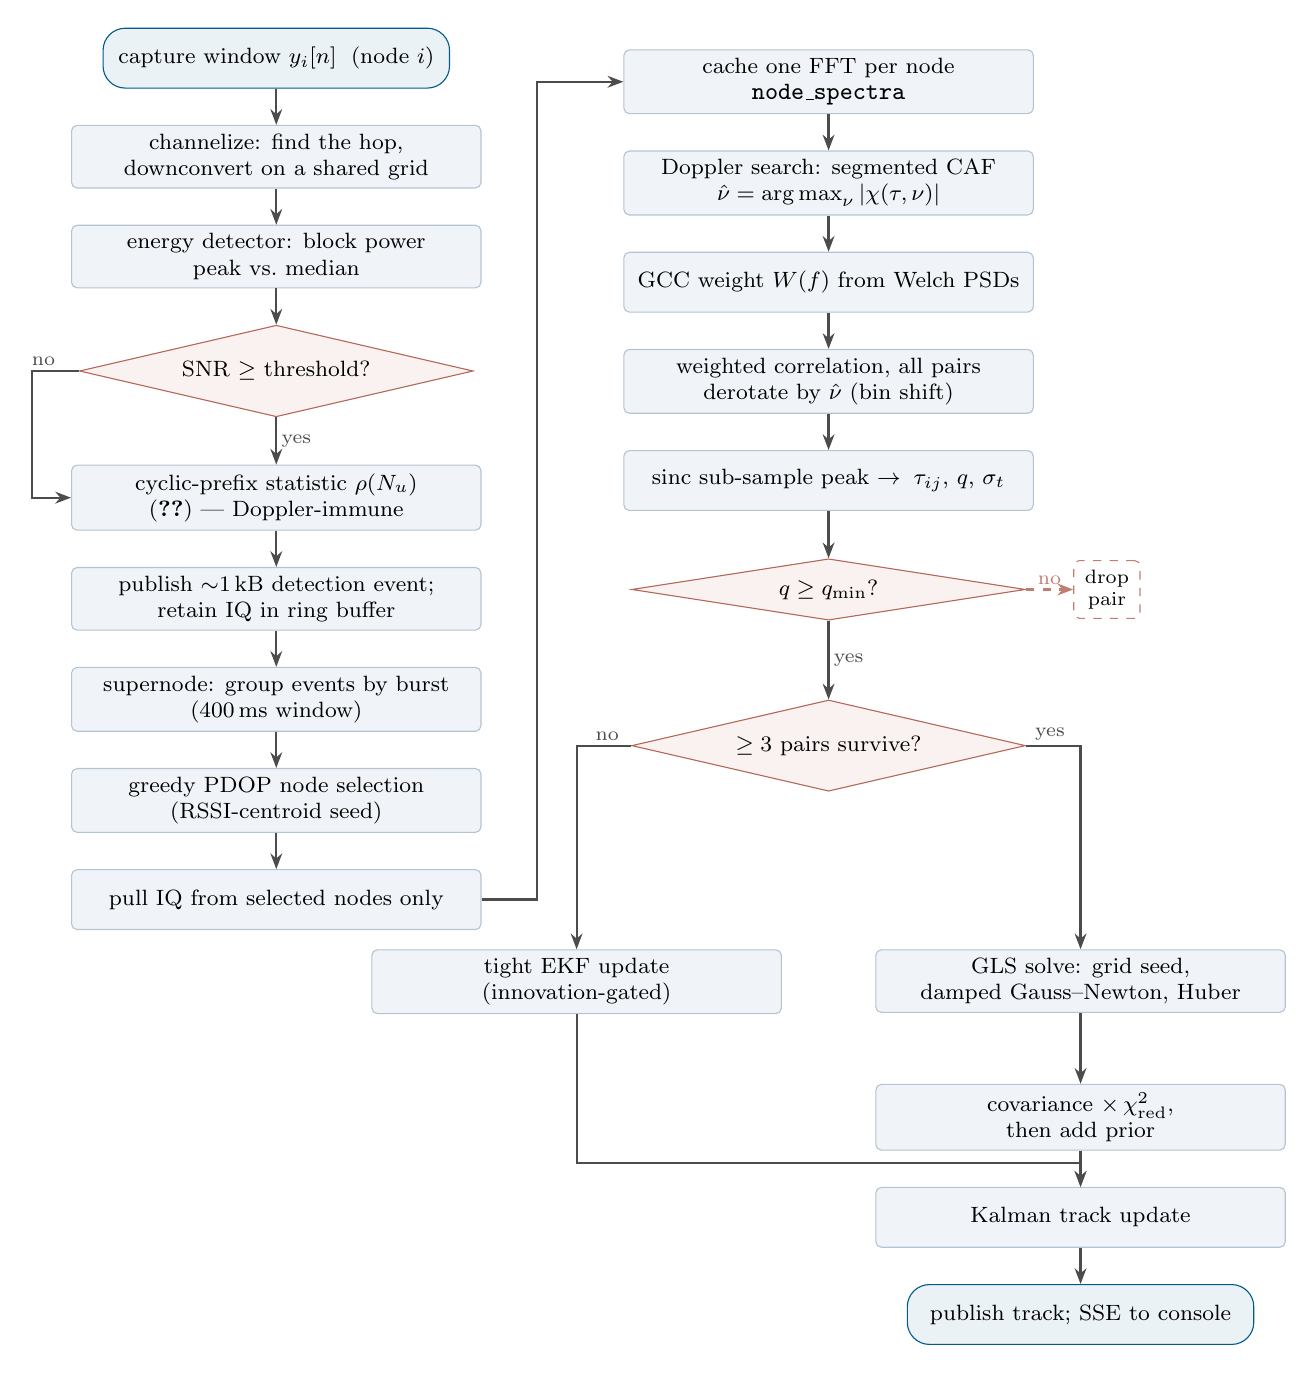
\begin{tikzpicture}[
  font=\footnotesize,
  node distance=4.6mm,
  proc/.style={draw=softrule,fill=soft,rounded corners=2pt,
               minimum width=52mm,minimum height=7.6mm,align=center,inner sep=3pt},
  dec/.style={draw=warn!70,fill=warn!6,diamond,aspect=2.9,
              minimum width=50mm,align=center,inner sep=1pt},
  term/.style={draw=accent,fill=accent!8,rounded corners=8pt,
               minimum width=44mm,minimum height=7.6mm,align=center},
  drop/.style={draw=warn!60,fill=white,rounded corners=2pt,dashed,
               minimum height=6mm,inner xsep=4pt,align=center,font=\scriptsize},
  ar/.style={-{Stealth[length=2mm]},thick,black!70},
  dar/.style={-{Stealth[length=2mm]},thick,warn!60,dashed},
  lbl/.style={font=\scriptsize,inner sep=1.5pt},
]
\node[term] (rx) {capture window $y_i[n]$ \;(node $i$)};
\node[proc,below=of rx] (chan) {channelize: find the hop,\\
      downconvert on a shared grid};
\node[proc,below=of chan] (det) {energy detector: block power\\peak vs.\ median};
\node[dec,below=of det] (gate) {SNR $\ge$ threshold?};
\node[proc,below=6mm of gate] (cyc) {cyclic-prefix statistic $\rho(N_u)$\\
      \eqref{eq:cyclo} --- Doppler-immune};
\node[proc,below=of cyc] (evt) {publish $\sim$1\,kB detection event;\\
      retain IQ in ring buffer};
\node[proc,below=of evt] (grp) {supernode: group events by burst\\(400\,ms window)};
\node[proc,below=of grp] (sel) {greedy PDOP node selection\\(RSSI-centroid seed)};
\node[proc,below=of sel] (pull) {pull IQ from selected nodes only};

\node[proc,right=22mm of rx,yshift=-3mm] (fft) {cache one FFT per node\\
      \code{node\_spectra}};
\node[proc,below=of fft] (dop) {Doppler search: segmented CAF\\
      $\hat\nu=\argmax_\nu|\chi(\tau,\nu)|$};
\node[proc,below=of dop] (wgt) {GCC weight $W(f)$ from Welch PSDs};
\node[proc,below=of wgt] (corr) {weighted correlation, all pairs\\
      derotate by $\hat\nu$ (bin shift)};
\node[proc,below=of corr] (sub) {sinc sub-sample peak $\to\;\tau_{ij},\,q,\,\sigma_t$};
\node[dec,below=6mm of sub] (qg) {$q \ge q_{\min}$?};
\node[dec,below=10mm of qg] (enough) {$\ge 3$ pairs survive?};
\node[drop,right=6mm of qg.east] (dropp) {drop\\pair};

\node[proc,below=20mm of enough,xshift=-32mm] (tight) {tight EKF update\\(innovation-gated)};
\node[proc,below=20mm of enough,xshift=32mm] (solve) {GLS solve: grid seed,\\
      damped Gauss--Newton, Huber};
\node[proc,below=9mm of solve] (cov) {covariance $\times\,\chi^2_{\text{red}}$,\\then add prior};
\node[proc,below=of cov] (trk) {Kalman track update};
\node[term,below=of trk] (out) {publish track; SSE to console};

\draw[ar] (rx) -- (chan);
\draw[ar] (chan) -- (det);
\draw[ar] (det) -- (gate);
\draw[ar] (gate) -- node[lbl,right]{yes} (cyc);
\draw[ar] (cyc) -- (evt);
\draw[ar] (evt) -- (grp);
\draw[ar] (grp) -- (sel);
\draw[ar] (sel) -- (pull);
\draw[ar] (pull.east) -- ++(0.7,0) |- (fft.west);

\draw[ar] (gate.west) -- ++(-0.6,0)
      node[lbl,above,align=center,pos=0.75]{no} |- (cyc.west);

\draw[ar] (fft) -- (dop);
\draw[ar] (dop) -- (wgt);
\draw[ar] (wgt) -- (corr);
\draw[ar] (corr) -- (sub);
\draw[ar] (sub) -- (qg);
\draw[ar] (qg) -- node[lbl,right]{yes} (enough);
\draw[dar] (qg.east) -- node[lbl,above]{no} (dropp.west);
\draw[ar] (enough.west) -| node[lbl,pos=0.22,above]{no} (tight.north);
\draw[ar] (enough.east) -| node[lbl,pos=0.22,above]{yes} (solve.north);
\draw[ar] (solve) -- (cov);
\draw[ar] (cov) -- (trk);
\draw[ar] (tight.south) |- ($(trk.north)+(0,3mm)$) -- (trk.north);
\draw[ar] (trk) -- (out);
\end{tikzpicture}
\caption{Per-burst processing. The left column runs on each sensor node; the
right column runs on the supernode. Note the two recovery paths that a naive
pipeline would omit: a burst failing the energy gate is still admitted when
the cyclostationary statistic fires (Section~\ref{sec:cyclo}), and a burst
with too few surviving pairs to solve still updates an existing track
through the tightly coupled filter rather than being discarded.}
\label{fig:flow}
\end{figure}

%==================================================================
\section{Numerical conditioning}

Several of the largest accuracy gains in this system's history came not from
better algorithms but from removing arithmetic that destroyed information
before the algorithms ever saw it. They are collected here because they
generalise.

\subsection{Absolute timestamps in a difference}

The delay~\eqref{eq:delay} was originally formed by building an absolute
arrival instant $t_0 + r_i/c + \varepsilon_i$ and subtracting the capture
start afterwards. At $t\approx1.785\times10^{9}$\,s the spacing of
\texttt{float64} is
\begin{equation}
  \operatorname{ulp}(t) = 2^{\lfloor\log_2 t\rfloor - 52}
  \approx 2.38\times10^{-7}\,\text{s} = 238\,\text{ns}.
\end{equation}
Time of flight and clock error --- the quantities the entire system
exists to measure, both far smaller than $238$\,ns --- were therefore
rounded onto a $238$\,ns grid before the subtraction could recover them.
The cost was roughly $70$\,ns RMS per node, $100$\,ns between a pair, some
$30$\,m of range, discarded for nothing.

The fix is to form the difference of the two large, nearby epochs
\emph{first}, exactly as in~\eqref{eq:delay}: $(t_0-t_{\text{cap}})$ is
computed without loss because the operands are close, and every small
quantity is added afterwards.

\begin{keypoint}
\textbf{A synthetic test that starts its clock at zero cannot see this.} The
unit test used $t_0=0$, and so had no epoch magnitude to lose precision
against; it reported $0.8$\,ns residual while the live pipeline sat at
$58$\,ns. Any test of a timing system must run at realistic absolute times.
\end{keypoint}

\subsection{Drift anchored to the wrong epoch}

Accumulating oscillator drift from the Unix epoch rather than from session
start gives $\delta\times1.78\times10^{9}\,\text{s}\approx35$\,s of apparent
clock error. That is not a subtle inaccuracy: it turned a $10$\,ms capture
into an $85$-million-sample allocation and wedged the node's callback
thread. Drift must accumulate from a session reference.

\subsection{Evaluating a stochastic model twice}

Under the disciplined-clock model the error is a stateful process. Calling
the model a second time to populate event metadata therefore reported an
error the signal never had; the supernode subtracted the wrong number and
the difference was pure uncorrectable error of about $21$\,ns. A stochastic
model must be evaluated once per event and the value reused. The bug was
harmless under the older deterministic model, which is precisely why it
appeared the moment realism was added.

\subsection{Scoring against the wrong reference}

The error metric compared each fix against the most recently received
ground-truth message rather than the truth of the burst that fix solved.
Once solve latency exceeded the truth interval, the metric measured
\emph{latency}, not accuracy: at $31$\,m/s and two bursts per second a
$150$\,ms solve reads as $15.8$\,m of horizontal error that no solver change
can remove. The diagnostic tell was horizontal error exceeding vertical with
a healthy $\chi^2$ --- geometrically impossible for this constellation
(Section~\ref{sec:gdop}), and therefore a bug in the measurement of the
measurement.

\subsection{A window sized by the wrong bound}

Discussed in Section~\ref{sec:window}: sizing the correlation search by
geometry alone ignores that the peak also carries the clock offset
difference. This failure is \emph{time-dependent} --- a fresh run looks
perfect and degrades as drift accumulates --- so a short smoke test cannot
detect it. Measured after $26$ minutes of running: clock deltas reaching
$92\,\mu$s against a $27\,\mu$s window, all $104$ fixes overflowing,
$\chi^2_{\text{red}}\approx1.1\times10^{6}$, horizontal error $870$\,m.

%==================================================================
\section{Measured performance}
\label{sec:measured}

Ten emulated nodes, two bursts per second, CP-OFDM emitter, moving target,
disciplined clocks:

\begin{center}
\begin{tabular}{@{}lr@{}}
\toprule
\textbf{Quantity} & \textbf{Value}\\
\midrule
Aggregate ingest                          & 3.7--4.4\,Mbps\\
Correlate and solve (CPU, 21 weighted CAF pairs) & $\approx100$\,ms\\
Reduced chi-square, median                & 0.45\\
Horizontal error, median                  & 0.2\,m\\
Vertical error, median                    & $\approx2$\,m\\
Covariance containment (horizontal / vertical) & 62\,\% / 65\,\% (target 68\,\%)\\
\bottomrule
\end{tabular}
\end{center}

Selected controlled comparisons, each with everything else held fixed:

\begin{center}
\begin{tabular}{@{}lll@{}}
\toprule
\textbf{Change} & \textbf{Without} & \textbf{With}\\
\midrule
Sinc vs.\ parabolic interpolation & 0.081 samp.\ RMS & 0.0017 samp.\ RMS\\
CAF on a moving emitter (per pair) & 26.7\,ns worst & 1.4\,ns worst\\
CAF, full solve                    & 1.7\,m, $\chi^2\!=\!5.0$ & 0.2\,m, $\chi^2\!=\!0.37$\\
All-pairs GLS vs.\ star reference  & 4.33\,m mean & 3.54\,m mean\\
Robust loss, one corrupted node    & 330.6\,m & 8.9\,m\\
GCC weighting, node-local interference & 8.9\,ns RMS & 3.5\,ns RMS\\
GCC weighting, fleet (defences off)    & 31.1\,m & 2.3\,m\\
GCC weighting, fleet (defences on, p90)& 3.19\,m & 0.56\,m\\
Cyclostationary vs.\ energy detection  & $+8$\,dB & $-2$\,dB\\
Channelizer vs.\ hopping emitter (detection) & 1 of 16 & 16 of 16\\
Bandwidth under multipath ($2\to18$\,MHz) & 4.57\,m & 0.26\,m\\
Robust loss under multipath (no outlier) & 4.57\,m & 4.50\,m\\
\bottomrule
\end{tabular}
\end{center}

Two of these deserve comment, in opposite directions.

Weighting's apparent value depends entirely on what else is running: in
isolation it rescues a fix from $31$\,m to $2.3$\,m, but with the quality
gate, robust loss and all-pairs GLS already absorbing single-pair damage,
its contribution shrinks to a tail effect. Reporting the isolated figure as
the system benefit would be dishonest.

The last row is a null result and is listed deliberately. Robust loss is
the strongest defence in this document against a corrupted node
($330.6\to8.9$\,m) and is worth nothing at all against multipath, because
one failure is an outlier and the other is common-mode. A table of
improvements that omitted the case where a technique does nothing would
misrepresent when to reach for it.

\paragraph{Note on comparability.} The headline figures above are measured
against a simulator that models the carrier, emitter motion, disciplined
clock noise and a structured OFDM waveform. Earlier revisions of this
system reported $0.4$\,m horizontal against a baseband-only simulator with
a spectrally flat emitter. The current numbers are therefore not merely
better; they are obtained under conditions the earlier configuration would
not have survived --- with the carrier modelled and the cross-ambiguity
search disabled, the same fleet degrades to $1.7$\,m and
$\chi^2_{\text{red}}=5.0$. Interference, hopping and multipath remain
disabled by default, and each is documented above with the cost of
enabling it.

\paragraph{A caution about where these numbers are taken.} Solve time is a
property of the machine as much as of the algorithm, and the failure mode
is worth stating because it is indistinguishable from a regression. On a
four-core mobile processor the full simulation --- twelve processes, plus a
browser drawing a city --- can drive the package to its thermal limit, at
which point the cores clock down to a fraction of nominal. Observed:
package at $96\,^\circ$C, cores pinned at $200$--$400$\,MHz against a
$4700$\,MHz maximum, and a $64$\,kB FFT taking $40$\,ms on an
\emph{otherwise idle} machine where it takes $1.2$\,ms cool --- a factor of
$34$. Solve time went from $86$\,ms to several seconds, the correlator fell
permanently behind the burst rate, and the tracker began correcting with
seconds-old fixes, which on screen looks exactly like a solver that has
lost its target.

The tell is that the degradation is \emph{uniform}: correlation, IQ
transfer and an unrelated numerical benchmark all slow by the same factor,
where a genuine regression is localised to whatever changed. The remedy is
to let the machine cool and re-measure, never to retune the estimator
against thermally-limited numbers. Cool, the same reduced configuration
sustains $86$--$93$\,ms with every burst solved.

%==================================================================
\section{First hardware: a TinyB210 on the bench}
\label{sec:hw}

Every number in \S\ref{sec:measured} comes from emulated nodes. This section
records what happened when a single real receiver --- a HamGeek TinyB210, a
B210 clone built on the AD9361 --- was attached, and separates what that
measurement established from what it could not.

\subsection{What the device reports}

\begin{center}
\small
\begin{tabular}{@{}ll@{}}
\toprule
Identity & \code{B210}, serial \code{271512}, EEPROM name \code{MyB210} \\
Firmware / FPGA & \code{8.0} / \code{16.0}, board revision 4, USB 3 \\
Discipline & \code{GPSTCXO v3.9 for TinyB210} \\
Clock sources & \code{internal}, \code{external}, \code{gpsdo} \\
Time sources & \code{none}, \code{internal}, \code{external}, \code{gpsdo} \\
Sensors & \code{gps\_gpgga}, \code{gps\_gprmc}, \code{gps\_time},
           \code{gps\_locked}, \code{gps\_servo}, \code{ref\_locked} \\
Receive & 2 channels, $50$--$6000$\,MHz, up to $56$\,MHz bandwidth \\
\bottomrule
\end{tabular}
\end{center}

That \code{gpsdo} appears as both a clock and a time source, and that
\code{gps\_locked} and \code{ref\_locked} exist as sensors, is the wiring TDOA
requires; a clone that had economised here would have been unusable. One detail
matters later: the discipline is a \emph{TCXO}, not an OCXO.

\subsection{What was verified without a GPS antenna}

\begin{center}
\small
\begin{tabular}{@{}lll@{}}
\toprule
\textbf{Property} & \textbf{Result} & \textbf{Bearing on the theory} \\
\midrule
Requested vs.\ actual rate & exact at $2.4$ and $20$\,Msps &
  a mismatch is a multiplicative bias on every TDOA \\
Requested vs.\ actual $f_c$ & exact at $2437$\,MHz & as above \\
Continuous $20$\,Msps, 2\,ch & $156$\,MB/s, no overflow &
  the wideband profile of \S\ref{sec:multipath} is affordable \\
Burst capture, isolated & clean, $8/8$ and $12/12$ &
  the capture primitive itself is sound \\
Under full node workload & clean at $2.4$\,Msps; intermittent
  overflow at $20$ & host-side contention, not a link ceiling \\
Channel coherence, no antenna & $0.030$ &
  independent noise, as \S\ref{sec:df} predicts \\
Channel coherence, 2 antennas & $0.59$ mean, $0.92$ peak &
  the interferometer of \S\ref{sec:df} is real \\
\bottomrule
\end{tabular}
\end{center}

Two results deserve emphasis. First, with two antennas the coherence between
channels rose by more than an order of magnitude, which is the physical
precondition for the two-element bearing estimate --- the phase difference is
meaningless if the channels are not coherent. Second, the cyclostationary
detector fired on genuine over-the-air Wi-Fi, classifying it \code{uas\_ofdm}
and retaining bursts down to $-7.8$\,dB SNR where the energy gate requires
$+8$\,dB. Wi-Fi is CP-OFDM, structurally what the detector was designed
against, so this is the first confirmation on a signal no simulation produced
that the $\sim\!10$\,dB margin claimed in \S\ref{sec:cyclo} is real.

\subsection{What changes when the GPSDO locks}

Without lock the device time source stays \code{internal}: device time counts
from power-on with no relation to UTC, \code{time\_aligned} is false, and
\code{node.py} refuses \code{capture.mode: scheduled} outright rather than
producing buffers that look simultaneous and are not. Four things change on
lock.

\paragraph{1. The device clock is stepped to UTC on a PPS edge.}
\code{set\_time\_next\_pps} --- not \code{set\_time\_now} --- writes the next
whole UTC second so that the device's notion of time advances on the
\emph{physical} pulse. All nodes then agree to within their PPS accuracy rather
than to within host scheduling jitter, which is hundreds of microseconds and
would dominate everything in \S\ref{sec:tde}.

\paragraph{2. Scheduled capture becomes legal, and needs no coordination.}
Each node derives its capture instants from UTC alone,
$t_k = k/f_{\text{burst}}$, so independently started nodes open the same window
without exchanging a message; the slot index doubles as the burst id the
supernode groups on. This replaces the bench fallback in which every node
free-runs and inter-node TDOA is meaningless.

\paragraph{3. Frequency discipline bounds the correlation window.} This is the
quantitative one. Two oscillators with fractional frequency error
$\Delta f/f$ accumulate relative timing offset
\begin{equation}
\Delta t(T) \;=\; \frac{\Delta f}{f}\,T ,
\label{eq:drift}
\end{equation}
and the correlation peak sits at geometric TDOA \emph{plus} that offset, of
which only the first term is bounded by the array baseline. With a
$\pm 5$\,km baseline the geometric term is under $\pm 17\,\mu$s and the search
window is $\sim\!27\,\mu$s; \eqref{eq:drift} says how long each discipline mode
keeps the true peak inside it:

\begin{center}
\small
\begin{tabular}{@{}llr@{}}
\toprule
\textbf{Mode} & \textbf{Typical $\Delta f/f$} & \textbf{Time to exceed $27\,\mu$s} \\
\midrule
\code{free} (undisciplined TCXO)  & $10^{-6}$   & $\sim\!27$\,s \\
\code{holdover} (TCXO, post-lock) & $10^{-7}$   & $\sim\!4.5$\,min \\
\code{gpsdo} (locked)             & $10^{-11}$  & $\sim\!31$\,days \\
\bottomrule
\end{tabular}
\end{center}

\noindent
These are order-of-magnitude figures from oscillator specifications, not
measurements of this board. The structure is what matters: GPS lock is what
makes a \emph{narrow} correlation window sustainable, and a narrow window is
what buys the sidelobe rejection that \S\ref{sec:window} shows cannot simply be
traded away by widening the search.

\begin{keypoint}
This is the same failure recorded in \S\ref{sec:window}, seen from the clock
side. It is also why \code{holdover} on \emph{this} board deserves its own
measurement: the discipline is a TCXO, and a TCXO's holdover is roughly an
order of magnitude worse than the OCXO the mode name suggests. Losing GPS on
this hardware is a matter of minutes before the window overflows, not hours.
\end{keypoint}

\paragraph{4. The schedule error becomes observable.} With a common UTC grid,
the per-capture quantity
$\text{clk\_off} = -(t_{0,\text{actual}} - t_{\text{slot}})$ is the hardware's
own report of how far its capture landed from the instant requested, and
\code{sched\_err\_ns} --- currently null --- is populated. Its
\emph{standard deviation} across captures is the jitter figure below.

\subsection{What remains unmeasured}

The decisive number is untouched. A \emph{constant} schedule offset is common
to all nodes and cancels in the difference \eqref{eq:tdoa}; the
\emph{jitter} does not, and enters the solution as timing noise amplified by
geometry. At the dilution figures of \S\ref{sec:gdop} a jitter of $\sigma_t$
contributes roughly $\text{VDOP}\cdot c\,\sigma_t$ to vertical error, so
$50$\,ns of jitter is already $\sim\!240$\,m of vertical uncertainty before
anything else is counted. That is why the acceptance threshold is where it is,
and it cannot be evaluated without an antenna that can see the sky.

\section{Limits}

\paragraph{Emission is required.} Everything here localizes emitters.
Non-cooperative is not the same as non-emitting: consumer drones stream
video continuously, which is why this approach is viable at all. A fully
radio-silent autonomous drone is invisible to TDOA, to direction finding,
and to the cross-ambiguity function alike. That regime needs passive radar
against broadcast illuminators, acoustics, or electro-optical sensing.

That fallback is a different band, not merely a different mode. A
$10$-inch carbon-fibre propeller resonates as a half-wave dipole near
$600$\,MHz, measured drone radar cross-section peaks there and falls some
$6$\,dB by $1$\,GHz, and every published passive detection of a small drone
uses a UHF illuminator --- DVB-T, DAB or LTE450, roughly $450$--$770$\,MHz
--- never the $2.4$\,GHz band this system operates in. Reported ranges are
$0.5$--$3$\,km against small airframes, the outlier being $5$\,km with a
$50$\,kW transmitter; median airframe RCS is $-20$ to $-15$\,dBsm with a
further $5$--$9$\,dB of fluctuation loss. Any such extension therefore needs
its own antennas, its own receive chain, and a direct-path canceller ---
the direct signal runs roughly $40$\,dB above the target return --- none of
which is shared with the emitter-localization path described here.

\paragraph{Node survey error propagates one-to-one.} A single GNSS fix is
accurate to $3$--$5$\,m, and node position error enters the solution
directly. Real deployment requires RTK or a 24-hour static survey.

\paragraph{Clock error is systematic, not noise.} The chi-square scaling
in~\eqref{eq:cov} honestly inflates covariance for random error but still
under-reports bias-driven error. An uncalibrated deployment produces a
confident, stable, wrong solution --- the most dangerous failure mode
available.

\paragraph{Detection thresholds are synthetic.} The cyclostationary
threshold and the classification boundary are set against simulated data.
Their mechanics are proven; the constants require real band captures.

\paragraph{Single target.} See data association above.

\paragraph{Hardware timing is still unmeasured.} \S\ref{sec:hw} closed part of
this gap and not the decisive part. A real TinyB210 now streams at both
profile rates without loss, tunes and samples at exactly the requested
parameters, and produces coherent dual-channel data and genuine
cyclostationary detections. What it has not done is lock its GPSDO, because
that needs an antenna with sky view --- so the schedule jitter remains
unquantified. A constant offset is common to all nodes and cancels
in~\eqref{eq:tdoa}; jitter does not. Below $50$\,ns the approach is viable;
above $200$\,ns the timing path is unusable for TDOA and the hardware is
useful only for direction finding. No amount of the mathematics in this
document changes that number.

\paragraph{One receiver is not a fix.} A single node contributes zero TDOA
rows: the measurement is a \emph{difference} between nodes, and
$\text{min\_nodes}=5$ is a property of the geometry, not a configurable
convenience. Bench work with one radio can validate the signal chain, the
detector, the bearing estimate and the transport, and can validate nothing
about localization.

\end{document}
